\documentclass[11pt]{article}

    \usepackage[breakable]{tcolorbox}
    \usepackage{parskip} % Stop auto-indenting (to mimic markdown behaviour)
    
    \usepackage{iftex}
    \ifPDFTeX
    	\usepackage[T1]{fontenc}
    	\usepackage{mathpazo}
    \else
    	\usepackage{fontspec}
    \fi

    % Basic figure setup, for now with no caption control since it's done
    % automatically by Pandoc (which extracts ![](path) syntax from Markdown).
    \usepackage{graphicx}
    % Maintain compatibility with old templates. Remove in nbconvert 6.0
    \let\Oldincludegraphics\includegraphics
    % Ensure that by default, figures have no caption (until we provide a
    % proper Figure object with a Caption API and a way to capture that
    % in the conversion process - todo).
    \usepackage{caption}
    \DeclareCaptionFormat{nocaption}{}
    \captionsetup{format=nocaption,aboveskip=0pt,belowskip=0pt}

    \usepackage[Export]{adjustbox} % Used to constrain images to a maximum size
    \adjustboxset{max size={0.9\linewidth}{0.9\paperheight}}
    \usepackage{float}
    \floatplacement{figure}{H} % forces figures to be placed at the correct location
    \usepackage{xcolor} % Allow colors to be defined
    \usepackage{enumerate} % Needed for markdown enumerations to work
    \usepackage{geometry} % Used to adjust the document margins
    \usepackage{amsmath} % Equations
    \usepackage{amssymb} % Equations
    \usepackage{textcomp} % defines textquotesingle
    % Hack from http://tex.stackexchange.com/a/47451/13684:
    \AtBeginDocument{%
        \def\PYZsq{\textquotesingle}% Upright quotes in Pygmentized code
    }
    \usepackage{upquote} % Upright quotes for verbatim code
    \usepackage{eurosym} % defines \euro
    \usepackage[mathletters]{ucs} % Extended unicode (utf-8) support
    \usepackage{fancyvrb} % verbatim replacement that allows latex
    \usepackage{grffile} % extends the file name processing of package graphics 
                         % to support a larger range
    \makeatletter % fix for grffile with XeLaTeX
    \def\Gread@@xetex#1{%
      \IfFileExists{"\Gin@base".bb}%
      {\Gread@eps{\Gin@base.bb}}%
      {\Gread@@xetex@aux#1}%
    }
    \makeatother

    % The hyperref package gives us a pdf with properly built
    % internal navigation ('pdf bookmarks' for the table of contents,
    % internal cross-reference links, web links for URLs, etc.)
    \usepackage{hyperref}
    % The default LaTeX title has an obnoxious amount of whitespace. By default,
    % titling removes some of it. It also provides customization options.
    \usepackage{titling}
    \usepackage{longtable} % longtable support required by pandoc >1.10
    \usepackage{booktabs}  % table support for pandoc > 1.12.2
    \usepackage[inline]{enumitem} % IRkernel/repr support (it uses the enumerate* environment)
    \usepackage[normalem]{ulem} % ulem is needed to support strikethroughs (\sout)
                                % normalem makes italics be italics, not underlines
    \usepackage{mathrsfs}
    

    
    % Colors for the hyperref package
    \definecolor{urlcolor}{rgb}{0,.145,.698}
    \definecolor{linkcolor}{rgb}{.71,0.21,0.01}
    \definecolor{citecolor}{rgb}{.12,.54,.11}

    % ANSI colors
    \definecolor{ansi-black}{HTML}{3E424D}
    \definecolor{ansi-black-intense}{HTML}{282C36}
    \definecolor{ansi-red}{HTML}{E75C58}
    \definecolor{ansi-red-intense}{HTML}{B22B31}
    \definecolor{ansi-green}{HTML}{00A250}
    \definecolor{ansi-green-intense}{HTML}{007427}
    \definecolor{ansi-yellow}{HTML}{DDB62B}
    \definecolor{ansi-yellow-intense}{HTML}{B27D12}
    \definecolor{ansi-blue}{HTML}{208FFB}
    \definecolor{ansi-blue-intense}{HTML}{0065CA}
    \definecolor{ansi-magenta}{HTML}{D160C4}
    \definecolor{ansi-magenta-intense}{HTML}{A03196}
    \definecolor{ansi-cyan}{HTML}{60C6C8}
    \definecolor{ansi-cyan-intense}{HTML}{258F8F}
    \definecolor{ansi-white}{HTML}{C5C1B4}
    \definecolor{ansi-white-intense}{HTML}{A1A6B2}
    \definecolor{ansi-default-inverse-fg}{HTML}{FFFFFF}
    \definecolor{ansi-default-inverse-bg}{HTML}{000000}

    % commands and environments needed by pandoc snippets
    % extracted from the output of `pandoc -s`
    \providecommand{\tightlist}{%
      \setlength{\itemsep}{0pt}\setlength{\parskip}{0pt}}
    \DefineVerbatimEnvironment{Highlighting}{Verbatim}{commandchars=\\\{\}}
    % Add ',fontsize=\small' for more characters per line
    \newenvironment{Shaded}{}{}
    \newcommand{\KeywordTok}[1]{\textcolor[rgb]{0.00,0.44,0.13}{\textbf{{#1}}}}
    \newcommand{\DataTypeTok}[1]{\textcolor[rgb]{0.56,0.13,0.00}{{#1}}}
    \newcommand{\DecValTok}[1]{\textcolor[rgb]{0.25,0.63,0.44}{{#1}}}
    \newcommand{\BaseNTok}[1]{\textcolor[rgb]{0.25,0.63,0.44}{{#1}}}
    \newcommand{\FloatTok}[1]{\textcolor[rgb]{0.25,0.63,0.44}{{#1}}}
    \newcommand{\CharTok}[1]{\textcolor[rgb]{0.25,0.44,0.63}{{#1}}}
    \newcommand{\StringTok}[1]{\textcolor[rgb]{0.25,0.44,0.63}{{#1}}}
    \newcommand{\CommentTok}[1]{\textcolor[rgb]{0.38,0.63,0.69}{\textit{{#1}}}}
    \newcommand{\OtherTok}[1]{\textcolor[rgb]{0.00,0.44,0.13}{{#1}}}
    \newcommand{\AlertTok}[1]{\textcolor[rgb]{1.00,0.00,0.00}{\textbf{{#1}}}}
    \newcommand{\FunctionTok}[1]{\textcolor[rgb]{0.02,0.16,0.49}{{#1}}}
    \newcommand{\RegionMarkerTok}[1]{{#1}}
    \newcommand{\ErrorTok}[1]{\textcolor[rgb]{1.00,0.00,0.00}{\textbf{{#1}}}}
    \newcommand{\NormalTok}[1]{{#1}}
    
    % Additional commands for more recent versions of Pandoc
    \newcommand{\ConstantTok}[1]{\textcolor[rgb]{0.53,0.00,0.00}{{#1}}}
    \newcommand{\SpecialCharTok}[1]{\textcolor[rgb]{0.25,0.44,0.63}{{#1}}}
    \newcommand{\VerbatimStringTok}[1]{\textcolor[rgb]{0.25,0.44,0.63}{{#1}}}
    \newcommand{\SpecialStringTok}[1]{\textcolor[rgb]{0.73,0.40,0.53}{{#1}}}
    \newcommand{\ImportTok}[1]{{#1}}
    \newcommand{\DocumentationTok}[1]{\textcolor[rgb]{0.73,0.13,0.13}{\textit{{#1}}}}
    \newcommand{\AnnotationTok}[1]{\textcolor[rgb]{0.38,0.63,0.69}{\textbf{\textit{{#1}}}}}
    \newcommand{\CommentVarTok}[1]{\textcolor[rgb]{0.38,0.63,0.69}{\textbf{\textit{{#1}}}}}
    \newcommand{\VariableTok}[1]{\textcolor[rgb]{0.10,0.09,0.49}{{#1}}}
    \newcommand{\ControlFlowTok}[1]{\textcolor[rgb]{0.00,0.44,0.13}{\textbf{{#1}}}}
    \newcommand{\OperatorTok}[1]{\textcolor[rgb]{0.40,0.40,0.40}{{#1}}}
    \newcommand{\BuiltInTok}[1]{{#1}}
    \newcommand{\ExtensionTok}[1]{{#1}}
    \newcommand{\PreprocessorTok}[1]{\textcolor[rgb]{0.74,0.48,0.00}{{#1}}}
    \newcommand{\AttributeTok}[1]{\textcolor[rgb]{0.49,0.56,0.16}{{#1}}}
    \newcommand{\InformationTok}[1]{\textcolor[rgb]{0.38,0.63,0.69}{\textbf{\textit{{#1}}}}}
    \newcommand{\WarningTok}[1]{\textcolor[rgb]{0.38,0.63,0.69}{\textbf{\textit{{#1}}}}}
    
    
    % Define a nice break command that doesn't care if a line doesn't already
    % exist.
    \def\br{\hspace*{\fill} \\* }
    % Math Jax compatibility definitions
    \def\gt{>}
    \def\lt{<}
    \let\Oldtex\TeX
    \let\Oldlatex\LaTeX
    \renewcommand{\TeX}{\textrm{\Oldtex}}
    \renewcommand{\LaTeX}{\textrm{\Oldlatex}}
    % Document parameters
    % Document title
    \title{Comparing numerical results with experimental data}
    
    
    
    
    
% Pygments definitions
\makeatletter
\def\PY@reset{\let\PY@it=\relax \let\PY@bf=\relax%
    \let\PY@ul=\relax \let\PY@tc=\relax%
    \let\PY@bc=\relax \let\PY@ff=\relax}
\def\PY@tok#1{\csname PY@tok@#1\endcsname}
\def\PY@toks#1+{\ifx\relax#1\empty\else%
    \PY@tok{#1}\expandafter\PY@toks\fi}
\def\PY@do#1{\PY@bc{\PY@tc{\PY@ul{%
    \PY@it{\PY@bf{\PY@ff{#1}}}}}}}
\def\PY#1#2{\PY@reset\PY@toks#1+\relax+\PY@do{#2}}

\expandafter\def\csname PY@tok@w\endcsname{\def\PY@tc##1{\textcolor[rgb]{0.73,0.73,0.73}{##1}}}
\expandafter\def\csname PY@tok@c\endcsname{\let\PY@it=\textit\def\PY@tc##1{\textcolor[rgb]{0.25,0.50,0.50}{##1}}}
\expandafter\def\csname PY@tok@cp\endcsname{\def\PY@tc##1{\textcolor[rgb]{0.74,0.48,0.00}{##1}}}
\expandafter\def\csname PY@tok@k\endcsname{\let\PY@bf=\textbf\def\PY@tc##1{\textcolor[rgb]{0.00,0.50,0.00}{##1}}}
\expandafter\def\csname PY@tok@kp\endcsname{\def\PY@tc##1{\textcolor[rgb]{0.00,0.50,0.00}{##1}}}
\expandafter\def\csname PY@tok@kt\endcsname{\def\PY@tc##1{\textcolor[rgb]{0.69,0.00,0.25}{##1}}}
\expandafter\def\csname PY@tok@o\endcsname{\def\PY@tc##1{\textcolor[rgb]{0.40,0.40,0.40}{##1}}}
\expandafter\def\csname PY@tok@ow\endcsname{\let\PY@bf=\textbf\def\PY@tc##1{\textcolor[rgb]{0.67,0.13,1.00}{##1}}}
\expandafter\def\csname PY@tok@nb\endcsname{\def\PY@tc##1{\textcolor[rgb]{0.00,0.50,0.00}{##1}}}
\expandafter\def\csname PY@tok@nf\endcsname{\def\PY@tc##1{\textcolor[rgb]{0.00,0.00,1.00}{##1}}}
\expandafter\def\csname PY@tok@nc\endcsname{\let\PY@bf=\textbf\def\PY@tc##1{\textcolor[rgb]{0.00,0.00,1.00}{##1}}}
\expandafter\def\csname PY@tok@nn\endcsname{\let\PY@bf=\textbf\def\PY@tc##1{\textcolor[rgb]{0.00,0.00,1.00}{##1}}}
\expandafter\def\csname PY@tok@ne\endcsname{\let\PY@bf=\textbf\def\PY@tc##1{\textcolor[rgb]{0.82,0.25,0.23}{##1}}}
\expandafter\def\csname PY@tok@nv\endcsname{\def\PY@tc##1{\textcolor[rgb]{0.10,0.09,0.49}{##1}}}
\expandafter\def\csname PY@tok@no\endcsname{\def\PY@tc##1{\textcolor[rgb]{0.53,0.00,0.00}{##1}}}
\expandafter\def\csname PY@tok@nl\endcsname{\def\PY@tc##1{\textcolor[rgb]{0.63,0.63,0.00}{##1}}}
\expandafter\def\csname PY@tok@ni\endcsname{\let\PY@bf=\textbf\def\PY@tc##1{\textcolor[rgb]{0.60,0.60,0.60}{##1}}}
\expandafter\def\csname PY@tok@na\endcsname{\def\PY@tc##1{\textcolor[rgb]{0.49,0.56,0.16}{##1}}}
\expandafter\def\csname PY@tok@nt\endcsname{\let\PY@bf=\textbf\def\PY@tc##1{\textcolor[rgb]{0.00,0.50,0.00}{##1}}}
\expandafter\def\csname PY@tok@nd\endcsname{\def\PY@tc##1{\textcolor[rgb]{0.67,0.13,1.00}{##1}}}
\expandafter\def\csname PY@tok@s\endcsname{\def\PY@tc##1{\textcolor[rgb]{0.73,0.13,0.13}{##1}}}
\expandafter\def\csname PY@tok@sd\endcsname{\let\PY@it=\textit\def\PY@tc##1{\textcolor[rgb]{0.73,0.13,0.13}{##1}}}
\expandafter\def\csname PY@tok@si\endcsname{\let\PY@bf=\textbf\def\PY@tc##1{\textcolor[rgb]{0.73,0.40,0.53}{##1}}}
\expandafter\def\csname PY@tok@se\endcsname{\let\PY@bf=\textbf\def\PY@tc##1{\textcolor[rgb]{0.73,0.40,0.13}{##1}}}
\expandafter\def\csname PY@tok@sr\endcsname{\def\PY@tc##1{\textcolor[rgb]{0.73,0.40,0.53}{##1}}}
\expandafter\def\csname PY@tok@ss\endcsname{\def\PY@tc##1{\textcolor[rgb]{0.10,0.09,0.49}{##1}}}
\expandafter\def\csname PY@tok@sx\endcsname{\def\PY@tc##1{\textcolor[rgb]{0.00,0.50,0.00}{##1}}}
\expandafter\def\csname PY@tok@m\endcsname{\def\PY@tc##1{\textcolor[rgb]{0.40,0.40,0.40}{##1}}}
\expandafter\def\csname PY@tok@gh\endcsname{\let\PY@bf=\textbf\def\PY@tc##1{\textcolor[rgb]{0.00,0.00,0.50}{##1}}}
\expandafter\def\csname PY@tok@gu\endcsname{\let\PY@bf=\textbf\def\PY@tc##1{\textcolor[rgb]{0.50,0.00,0.50}{##1}}}
\expandafter\def\csname PY@tok@gd\endcsname{\def\PY@tc##1{\textcolor[rgb]{0.63,0.00,0.00}{##1}}}
\expandafter\def\csname PY@tok@gi\endcsname{\def\PY@tc##1{\textcolor[rgb]{0.00,0.63,0.00}{##1}}}
\expandafter\def\csname PY@tok@gr\endcsname{\def\PY@tc##1{\textcolor[rgb]{1.00,0.00,0.00}{##1}}}
\expandafter\def\csname PY@tok@ge\endcsname{\let\PY@it=\textit}
\expandafter\def\csname PY@tok@gs\endcsname{\let\PY@bf=\textbf}
\expandafter\def\csname PY@tok@gp\endcsname{\let\PY@bf=\textbf\def\PY@tc##1{\textcolor[rgb]{0.00,0.00,0.50}{##1}}}
\expandafter\def\csname PY@tok@go\endcsname{\def\PY@tc##1{\textcolor[rgb]{0.53,0.53,0.53}{##1}}}
\expandafter\def\csname PY@tok@gt\endcsname{\def\PY@tc##1{\textcolor[rgb]{0.00,0.27,0.87}{##1}}}
\expandafter\def\csname PY@tok@err\endcsname{\def\PY@bc##1{\setlength{\fboxsep}{0pt}\fcolorbox[rgb]{1.00,0.00,0.00}{1,1,1}{\strut ##1}}}
\expandafter\def\csname PY@tok@kc\endcsname{\let\PY@bf=\textbf\def\PY@tc##1{\textcolor[rgb]{0.00,0.50,0.00}{##1}}}
\expandafter\def\csname PY@tok@kd\endcsname{\let\PY@bf=\textbf\def\PY@tc##1{\textcolor[rgb]{0.00,0.50,0.00}{##1}}}
\expandafter\def\csname PY@tok@kn\endcsname{\let\PY@bf=\textbf\def\PY@tc##1{\textcolor[rgb]{0.00,0.50,0.00}{##1}}}
\expandafter\def\csname PY@tok@kr\endcsname{\let\PY@bf=\textbf\def\PY@tc##1{\textcolor[rgb]{0.00,0.50,0.00}{##1}}}
\expandafter\def\csname PY@tok@bp\endcsname{\def\PY@tc##1{\textcolor[rgb]{0.00,0.50,0.00}{##1}}}
\expandafter\def\csname PY@tok@fm\endcsname{\def\PY@tc##1{\textcolor[rgb]{0.00,0.00,1.00}{##1}}}
\expandafter\def\csname PY@tok@vc\endcsname{\def\PY@tc##1{\textcolor[rgb]{0.10,0.09,0.49}{##1}}}
\expandafter\def\csname PY@tok@vg\endcsname{\def\PY@tc##1{\textcolor[rgb]{0.10,0.09,0.49}{##1}}}
\expandafter\def\csname PY@tok@vi\endcsname{\def\PY@tc##1{\textcolor[rgb]{0.10,0.09,0.49}{##1}}}
\expandafter\def\csname PY@tok@vm\endcsname{\def\PY@tc##1{\textcolor[rgb]{0.10,0.09,0.49}{##1}}}
\expandafter\def\csname PY@tok@sa\endcsname{\def\PY@tc##1{\textcolor[rgb]{0.73,0.13,0.13}{##1}}}
\expandafter\def\csname PY@tok@sb\endcsname{\def\PY@tc##1{\textcolor[rgb]{0.73,0.13,0.13}{##1}}}
\expandafter\def\csname PY@tok@sc\endcsname{\def\PY@tc##1{\textcolor[rgb]{0.73,0.13,0.13}{##1}}}
\expandafter\def\csname PY@tok@dl\endcsname{\def\PY@tc##1{\textcolor[rgb]{0.73,0.13,0.13}{##1}}}
\expandafter\def\csname PY@tok@s2\endcsname{\def\PY@tc##1{\textcolor[rgb]{0.73,0.13,0.13}{##1}}}
\expandafter\def\csname PY@tok@sh\endcsname{\def\PY@tc##1{\textcolor[rgb]{0.73,0.13,0.13}{##1}}}
\expandafter\def\csname PY@tok@s1\endcsname{\def\PY@tc##1{\textcolor[rgb]{0.73,0.13,0.13}{##1}}}
\expandafter\def\csname PY@tok@mb\endcsname{\def\PY@tc##1{\textcolor[rgb]{0.40,0.40,0.40}{##1}}}
\expandafter\def\csname PY@tok@mf\endcsname{\def\PY@tc##1{\textcolor[rgb]{0.40,0.40,0.40}{##1}}}
\expandafter\def\csname PY@tok@mh\endcsname{\def\PY@tc##1{\textcolor[rgb]{0.40,0.40,0.40}{##1}}}
\expandafter\def\csname PY@tok@mi\endcsname{\def\PY@tc##1{\textcolor[rgb]{0.40,0.40,0.40}{##1}}}
\expandafter\def\csname PY@tok@il\endcsname{\def\PY@tc##1{\textcolor[rgb]{0.40,0.40,0.40}{##1}}}
\expandafter\def\csname PY@tok@mo\endcsname{\def\PY@tc##1{\textcolor[rgb]{0.40,0.40,0.40}{##1}}}
\expandafter\def\csname PY@tok@ch\endcsname{\let\PY@it=\textit\def\PY@tc##1{\textcolor[rgb]{0.25,0.50,0.50}{##1}}}
\expandafter\def\csname PY@tok@cm\endcsname{\let\PY@it=\textit\def\PY@tc##1{\textcolor[rgb]{0.25,0.50,0.50}{##1}}}
\expandafter\def\csname PY@tok@cpf\endcsname{\let\PY@it=\textit\def\PY@tc##1{\textcolor[rgb]{0.25,0.50,0.50}{##1}}}
\expandafter\def\csname PY@tok@c1\endcsname{\let\PY@it=\textit\def\PY@tc##1{\textcolor[rgb]{0.25,0.50,0.50}{##1}}}
\expandafter\def\csname PY@tok@cs\endcsname{\let\PY@it=\textit\def\PY@tc##1{\textcolor[rgb]{0.25,0.50,0.50}{##1}}}

\def\PYZbs{\char`\\}
\def\PYZus{\char`\_}
\def\PYZob{\char`\{}
\def\PYZcb{\char`\}}
\def\PYZca{\char`\^}
\def\PYZam{\char`\&}
\def\PYZlt{\char`\<}
\def\PYZgt{\char`\>}
\def\PYZsh{\char`\#}
\def\PYZpc{\char`\%}
\def\PYZdl{\char`\$}
\def\PYZhy{\char`\-}
\def\PYZsq{\char`\'}
\def\PYZdq{\char`\"}
\def\PYZti{\char`\~}
% for compatibility with earlier versions
\def\PYZat{@}
\def\PYZlb{[}
\def\PYZrb{]}
\makeatother


    % For linebreaks inside Verbatim environment from package fancyvrb. 
    \makeatletter
        \newbox\Wrappedcontinuationbox 
        \newbox\Wrappedvisiblespacebox 
        \newcommand*\Wrappedvisiblespace {\textcolor{red}{\textvisiblespace}} 
        \newcommand*\Wrappedcontinuationsymbol {\textcolor{red}{\llap{\tiny$\m@th\hookrightarrow$}}} 
        \newcommand*\Wrappedcontinuationindent {3ex } 
        \newcommand*\Wrappedafterbreak {\kern\Wrappedcontinuationindent\copy\Wrappedcontinuationbox} 
        % Take advantage of the already applied Pygments mark-up to insert 
        % potential linebreaks for TeX processing. 
        %        {, <, #, %, $, ' and ": go to next line. 
        %        _, }, ^, &, >, - and ~: stay at end of broken line. 
        % Use of \textquotesingle for straight quote. 
        \newcommand*\Wrappedbreaksatspecials {% 
            \def\PYGZus{\discretionary{\char`\_}{\Wrappedafterbreak}{\char`\_}}% 
            \def\PYGZob{\discretionary{}{\Wrappedafterbreak\char`\{}{\char`\{}}% 
            \def\PYGZcb{\discretionary{\char`\}}{\Wrappedafterbreak}{\char`\}}}% 
            \def\PYGZca{\discretionary{\char`\^}{\Wrappedafterbreak}{\char`\^}}% 
            \def\PYGZam{\discretionary{\char`\&}{\Wrappedafterbreak}{\char`\&}}% 
            \def\PYGZlt{\discretionary{}{\Wrappedafterbreak\char`\<}{\char`\<}}% 
            \def\PYGZgt{\discretionary{\char`\>}{\Wrappedafterbreak}{\char`\>}}% 
            \def\PYGZsh{\discretionary{}{\Wrappedafterbreak\char`\#}{\char`\#}}% 
            \def\PYGZpc{\discretionary{}{\Wrappedafterbreak\char`\%}{\char`\%}}% 
            \def\PYGZdl{\discretionary{}{\Wrappedafterbreak\char`\$}{\char`\$}}% 
            \def\PYGZhy{\discretionary{\char`\-}{\Wrappedafterbreak}{\char`\-}}% 
            \def\PYGZsq{\discretionary{}{\Wrappedafterbreak\textquotesingle}{\textquotesingle}}% 
            \def\PYGZdq{\discretionary{}{\Wrappedafterbreak\char`\"}{\char`\"}}% 
            \def\PYGZti{\discretionary{\char`\~}{\Wrappedafterbreak}{\char`\~}}% 
        } 
        % Some characters . , ; ? ! / are not pygmentized. 
        % This macro makes them "active" and they will insert potential linebreaks 
        \newcommand*\Wrappedbreaksatpunct {% 
            \lccode`\~`\.\lowercase{\def~}{\discretionary{\hbox{\char`\.}}{\Wrappedafterbreak}{\hbox{\char`\.}}}% 
            \lccode`\~`\,\lowercase{\def~}{\discretionary{\hbox{\char`\,}}{\Wrappedafterbreak}{\hbox{\char`\,}}}% 
            \lccode`\~`\;\lowercase{\def~}{\discretionary{\hbox{\char`\;}}{\Wrappedafterbreak}{\hbox{\char`\;}}}% 
            \lccode`\~`\:\lowercase{\def~}{\discretionary{\hbox{\char`\:}}{\Wrappedafterbreak}{\hbox{\char`\:}}}% 
            \lccode`\~`\?\lowercase{\def~}{\discretionary{\hbox{\char`\?}}{\Wrappedafterbreak}{\hbox{\char`\?}}}% 
            \lccode`\~`\!\lowercase{\def~}{\discretionary{\hbox{\char`\!}}{\Wrappedafterbreak}{\hbox{\char`\!}}}% 
            \lccode`\~`\/\lowercase{\def~}{\discretionary{\hbox{\char`\/}}{\Wrappedafterbreak}{\hbox{\char`\/}}}% 
            \catcode`\.\active
            \catcode`\,\active 
            \catcode`\;\active
            \catcode`\:\active
            \catcode`\?\active
            \catcode`\!\active
            \catcode`\/\active 
            \lccode`\~`\~ 	
        }
    \makeatother

    \let\OriginalVerbatim=\Verbatim
    \makeatletter
    \renewcommand{\Verbatim}[1][1]{%
        %\parskip\z@skip
        \sbox\Wrappedcontinuationbox {\Wrappedcontinuationsymbol}%
        \sbox\Wrappedvisiblespacebox {\FV@SetupFont\Wrappedvisiblespace}%
        \def\FancyVerbFormatLine ##1{\hsize\linewidth
            \vtop{\raggedright\hyphenpenalty\z@\exhyphenpenalty\z@
                \doublehyphendemerits\z@\finalhyphendemerits\z@
                \strut ##1\strut}%
        }%
        % If the linebreak is at a space, the latter will be displayed as visible
        % space at end of first line, and a continuation symbol starts next line.
        % Stretch/shrink are however usually zero for typewriter font.
        \def\FV@Space {%
            \nobreak\hskip\z@ plus\fontdimen3\font minus\fontdimen4\font
            \discretionary{\copy\Wrappedvisiblespacebox}{\Wrappedafterbreak}
            {\kern\fontdimen2\font}%
        }%
        
        % Allow breaks at special characters using \PYG... macros.
        \Wrappedbreaksatspecials
        % Breaks at punctuation characters . , ; ? ! and / need catcode=\active 	
        \OriginalVerbatim[#1,codes*=\Wrappedbreaksatpunct]%
    }
    \makeatother

    % Exact colors from NB
    \definecolor{incolor}{HTML}{303F9F}
    \definecolor{outcolor}{HTML}{D84315}
    \definecolor{cellborder}{HTML}{CFCFCF}
    \definecolor{cellbackground}{HTML}{F7F7F7}
    
    % prompt
    \makeatletter
    \newcommand{\boxspacing}{\kern\kvtcb@left@rule\kern\kvtcb@boxsep}
    \makeatother
    \newcommand{\prompt}[4]{
        \ttfamily\llap{{\color{#2}[#3]:\hspace{3pt}#4}}\vspace{-\baselineskip}
    }
    

    
    % Prevent overflowing lines due to hard-to-break entities
    \sloppy 
    % Setup hyperref package
    \hypersetup{
      breaklinks=true,  % so long urls are correctly broken across lines
      colorlinks=true,
      urlcolor=urlcolor,
      linkcolor=linkcolor,
      citecolor=citecolor,
      }
    % Slightly bigger margins than the latex defaults
    
    \geometry{verbose,tmargin=1in,bmargin=1in,lmargin=1in,rmargin=1in}
    
    

\begin{document}
    
    \maketitle
    
    

    
    \tableofcontents 
\setcounter{section}{0}

    \hypertarget{bibliography-section}{%
\section{Bibliography section}\label{bibliography-section}}

    \bibliographystyle{alphadin}
\bibliography{ipython}

    \begin{tcolorbox}[breakable, size=fbox, boxrule=1pt, pad at break*=1mm,colback=cellbackground, colframe=cellborder]
\prompt{In}{incolor}{129}{\boxspacing}
\begin{Verbatim}[commandchars=\\\{\}]
\PY{k+kn}{from} \PY{n+nn}{part2} \PY{k+kn}{import} \PY{o}{*}

\PY{k}{def} \PY{n+nf}{create\PYZus{}grain\PYZus{}from\PYZus{}data}\PY{p}{(}\PY{n}{dF}\PY{p}{)}\PY{p}{:}
    \PY{k}{if} \PY{n+nb}{type}\PY{p}{(}\PY{n}{dF}\PY{p}{)}\PY{o}{==}\PY{n}{pd}\PY{o}{.}\PY{n}{Series}\PY{p}{:}
        \PY{n}{dF} \PY{o}{=} \PY{n}{pd}\PY{o}{.}\PY{n}{DataFrame}\PY{p}{(}\PY{p}{[}\PY{n}{dF}\PY{p}{]}\PY{p}{)}
        
    \PY{k}{if} \PY{n+nb}{len}\PY{p}{(}\PY{n}{dF}\PY{p}{[}\PY{l+s+s1}{\PYZsq{}}\PY{l+s+s1}{temp}\PY{l+s+s1}{\PYZsq{}}\PY{p}{]}\PY{o}{.}\PY{n}{unique}\PY{p}{(}\PY{p}{)}\PY{p}{)}\PY{o}{==}\PY{l+m+mi}{1}\PY{p}{:}
        \PY{n}{T\PYZus{}C} \PY{o}{=} \PY{n}{dF}\PY{p}{[}\PY{l+s+s1}{\PYZsq{}}\PY{l+s+s1}{temp}\PY{l+s+s1}{\PYZsq{}}\PY{p}{]}\PY{o}{.}\PY{n}{unique}\PY{p}{(}\PY{p}{)}\PY{p}{[}\PY{l+m+mi}{0}\PY{p}{]}
    \PY{k}{else}\PY{p}{:}
        \PY{k}{raise} \PY{n+ne}{Exception}\PY{p}{(}\PY{l+s+s1}{\PYZsq{}}\PY{l+s+s1}{Multiple paramters for one grain are invalid.}\PY{l+s+s1}{\PYZsq{}}\PY{p}{)}
    
    \PY{k}{if} \PY{n+nb}{len}\PY{p}{(}\PY{n}{dF}\PY{p}{[}\PY{l+s+s1}{\PYZsq{}}\PY{l+s+s1}{ND}\PY{l+s+s1}{\PYZsq{}}\PY{p}{]}\PY{o}{.}\PY{n}{unique}\PY{p}{(}\PY{p}{)}\PY{p}{)}\PY{o}{==}\PY{l+m+mi}{1}\PY{p}{:}
        \PY{n}{ND} \PY{o}{=} \PY{n}{dF}\PY{p}{[}\PY{l+s+s1}{\PYZsq{}}\PY{l+s+s1}{ND}\PY{l+s+s1}{\PYZsq{}}\PY{p}{]}\PY{o}{.}\PY{n}{unique}\PY{p}{(}\PY{p}{)}\PY{p}{[}\PY{l+m+mi}{0}\PY{p}{]}
    \PY{k}{else}\PY{p}{:}
        \PY{k}{raise} \PY{n+ne}{Exception}\PY{p}{(}\PY{l+s+s1}{\PYZsq{}}\PY{l+s+s1}{Multiple paramters for one grain are invalid.}\PY{l+s+s1}{\PYZsq{}}\PY{p}{)}
    
    \PY{k}{if} \PY{n+nb}{len}\PY{p}{(}\PY{n}{dF}\PY{p}{[}\PY{l+s+s1}{\PYZsq{}}\PY{l+s+s1}{mass\PYZus{}eff}\PY{l+s+s1}{\PYZsq{}}\PY{p}{]}\PY{o}{.}\PY{n}{unique}\PY{p}{(}\PY{p}{)}\PY{p}{)}\PY{o}{==}\PY{l+m+mi}{1}\PY{p}{:}
        \PY{n}{mass\PYZus{}e\PYZus{}eff\PYZus{}factor} \PY{o}{=} \PY{n}{dF}\PY{p}{[}\PY{l+s+s1}{\PYZsq{}}\PY{l+s+s1}{mass\PYZus{}eff}\PY{l+s+s1}{\PYZsq{}}\PY{p}{]}\PY{o}{.}\PY{n}{unique}\PY{p}{(}\PY{p}{)}\PY{p}{[}\PY{l+m+mi}{0}\PY{p}{]}\PY{o}{/}\PY{n}{CONST}\PY{o}{.}\PY{n}{MASS\PYZus{}E} 
    \PY{k}{else}\PY{p}{:}
        \PY{k}{raise} \PY{n+ne}{Exception}\PY{p}{(}\PY{l+s+s1}{\PYZsq{}}\PY{l+s+s1}{Multiple paramters for one grain are invalid.}\PY{l+s+s1}{\PYZsq{}}\PY{p}{)}
    
    \PY{k}{if} \PY{n+nb}{len}\PY{p}{(}\PY{n}{dF}\PY{p}{[}\PY{l+s+s1}{\PYZsq{}}\PY{l+s+s1}{R}\PY{l+s+s1}{\PYZsq{}}\PY{p}{]}\PY{o}{.}\PY{n}{unique}\PY{p}{(}\PY{p}{)}\PY{p}{)}\PY{o}{==}\PY{l+m+mi}{1}\PY{p}{:}
        \PY{n}{grainsize\PYZus{}radius} \PY{o}{=} \PY{n}{dF}\PY{p}{[}\PY{l+s+s1}{\PYZsq{}}\PY{l+s+s1}{R}\PY{l+s+s1}{\PYZsq{}}\PY{p}{]}\PY{o}{.}\PY{n}{unique}\PY{p}{(}\PY{p}{)}\PY{p}{[}\PY{l+m+mi}{0}\PY{p}{]}
    \PY{k}{else}\PY{p}{:}
        \PY{k}{raise} \PY{n+ne}{Exception}\PY{p}{(}\PY{l+s+s1}{\PYZsq{}}\PY{l+s+s1}{Multiple paramters for one grain are invalid.}\PY{l+s+s1}{\PYZsq{}}\PY{p}{)}
        

    

    \PY{n}{material} \PY{o}{=} \PY{n}{Material}\PY{p}{(}\PY{n}{T\PYZus{}C}\PY{p}{,}\PY{n}{ND}\PY{p}{)}
    \PY{n}{grain} \PY{o}{=} \PY{n}{Grain}\PY{p}{(}\PY{n}{grainsize\PYZus{}radius}\PY{o}{=}\PY{n}{grainsize\PYZus{}radius}\PY{p}{,}\PY{n}{material}\PY{o}{=}\PY{n}{material}\PY{p}{)}
    
    \PY{k}{return} \PY{n}{grain}
\end{Verbatim}
\end{tcolorbox}

    \hypertarget{data-from-the-publication}{%
\subsection{Data from the publication}\label{data-from-the-publication}}

    \begin{figure}
\centering
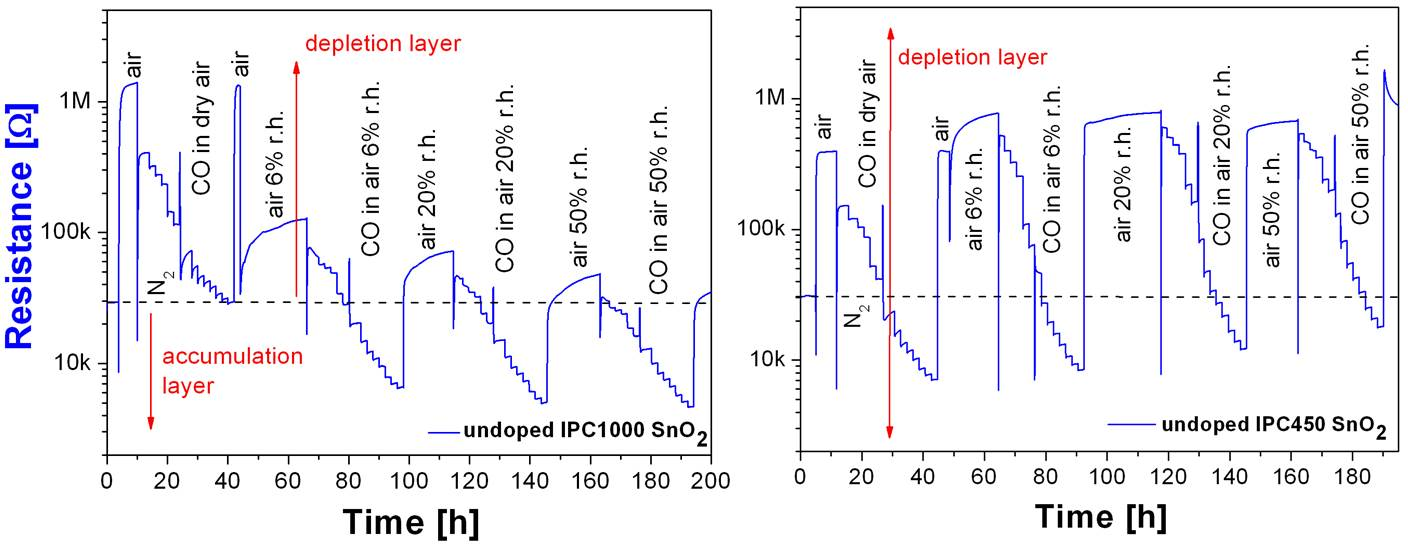
\includegraphics{media/rawdata450_1000.jpg}
\caption{test}
\end{figure}

    \hypertarget{import-the-experimental-results}{%
\section{Import the experimental
results}\label{import-the-experimental-results}}

    \begin{tcolorbox}[breakable, size=fbox, boxrule=1pt, pad at break*=1mm,colback=cellbackground, colframe=cellborder]
\prompt{In}{incolor}{130}{\boxspacing}
\begin{Verbatim}[commandchars=\\\{\}]
\PY{n}{calc\PYZus{}dF} \PY{o}{=} \PY{n}{pd}\PY{o}{.}\PY{n}{read\PYZus{}hdf}\PY{p}{(}\PY{l+s+s1}{\PYZsq{}}\PY{l+s+s1}{numerical\PYZus{}sol\PYZus{}2.h5}\PY{l+s+s1}{\PYZsq{}}\PY{p}{,}\PY{l+s+s1}{\PYZsq{}}\PY{l+s+s1}{raw}\PY{l+s+s1}{\PYZsq{}}\PY{p}{)}

\PY{n}{dF\PYZus{}450} \PY{o}{=} \PY{n}{pd}\PY{o}{.}\PY{n}{read\PYZus{}excel}\PY{p}{(}\PY{l+s+s1}{\PYZsq{}}\PY{l+s+s1}{Kelvin\PYZus{}Data.xlsx}\PY{l+s+s1}{\PYZsq{}}\PY{p}{,} \PY{n}{sheet\PYZus{}name}\PY{o}{=}\PY{l+s+s1}{\PYZsq{}}\PY{l+s+s1}{ipc450}\PY{l+s+s1}{\PYZsq{}}\PY{p}{)}\PY{o}{.}\PY{n}{sort\PYZus{}values}\PY{p}{(}\PY{n}{by}\PY{o}{=}\PY{l+s+s1}{\PYZsq{}}\PY{l+s+s1}{dV}\PY{l+s+s1}{\PYZsq{}}\PY{p}{)}
\PY{n}{dF\PYZus{}1000} \PY{o}{=} \PY{n}{pd}\PY{o}{.}\PY{n}{read\PYZus{}excel}\PY{p}{(}\PY{l+s+s1}{\PYZsq{}}\PY{l+s+s1}{Kelvin\PYZus{}Data.xlsx}\PY{l+s+s1}{\PYZsq{}}\PY{p}{,} \PY{n}{sheet\PYZus{}name}\PY{o}{=}\PY{l+s+s1}{\PYZsq{}}\PY{l+s+s1}{ipc1000}\PY{l+s+s1}{\PYZsq{}}\PY{p}{)}\PY{o}{.}\PY{n}{sort\PYZus{}values}\PY{p}{(}\PY{n}{by}\PY{o}{=}\PY{l+s+s1}{\PYZsq{}}\PY{l+s+s1}{dV}\PY{l+s+s1}{\PYZsq{}}\PY{p}{)}

\PY{n}{gs} \PY{o}{=} \PY{n}{calc\PYZus{}dF}\PY{o}{.}\PY{n}{groupby}\PY{p}{(}\PY{p}{[}\PY{l+s+s1}{\PYZsq{}}\PY{l+s+s1}{R}\PY{l+s+s1}{\PYZsq{}}\PY{p}{,}\PY{l+s+s1}{\PYZsq{}}\PY{l+s+s1}{ND}\PY{l+s+s1}{\PYZsq{}}\PY{p}{]}\PY{p}{)}
\end{Verbatim}
\end{tcolorbox}

    \begin{tcolorbox}[breakable, size=fbox, boxrule=1pt, pad at break*=1mm,colback=cellbackground, colframe=cellborder]
\prompt{In}{incolor}{131}{\boxspacing}
\begin{Verbatim}[commandchars=\\\{\}]
\PY{o}{\PYZpc{}}\PY{k}{pylab} qt5
\PY{o}{\PYZpc{}}\PY{k}{matplotlib} qt5
\end{Verbatim}
\end{tcolorbox}

    \begin{Verbatim}[commandchars=\\\{\}]
Populating the interactive namespace from numpy and matplotlib
    \end{Verbatim}

    \begin{Verbatim}[commandchars=\\\{\}]
/usr/lib/python3.8/site-packages/IPython/core/magics/pylab.py:159: UserWarning:
pylab import has clobbered these variables: ['interp', 'axes']
`\%matplotlib` prevents importing * from pylab and numpy
  warn("pylab import has clobbered these variables: \%s"  \% clobbered +
    \end{Verbatim}

    \begin{tcolorbox}[breakable, size=fbox, boxrule=1pt, pad at break*=1mm,colback=cellbackground, colframe=cellborder]
\prompt{In}{incolor}{132}{\boxspacing}
\begin{Verbatim}[commandchars=\\\{\}]
\PY{k+kn}{from} \PY{n+nn}{scipy}\PY{n+nn}{.}\PY{n+nn}{optimize} \PY{k+kn}{import} \PY{n}{curve\PYZus{}fit}
\end{Verbatim}
\end{tcolorbox}

    \begin{tcolorbox}[breakable, size=fbox, boxrule=1pt, pad at break*=1mm,colback=cellbackground, colframe=cellborder]
\prompt{In}{incolor}{133}{\boxspacing}
\begin{Verbatim}[commandchars=\\\{\}]
\PY{n}{fig}\PY{p}{,} \PY{n}{axe} \PY{o}{=} \PY{n}{subplots}\PY{p}{(}\PY{p}{)}
\PY{n}{axe}\PY{o}{.}\PY{n}{scatter}\PY{p}{(}\PY{n}{dF\PYZus{}450}\PY{p}{[}\PY{l+s+s1}{\PYZsq{}}\PY{l+s+s1}{dV}\PY{l+s+s1}{\PYZsq{}}\PY{p}{]}\PY{p}{,}\PY{n}{dF\PYZus{}450}\PY{p}{[}\PY{l+s+s1}{\PYZsq{}}\PY{l+s+s1}{res}\PY{l+s+s1}{\PYZsq{}}\PY{p}{]}\PY{p}{)}
\PY{n}{axe}\PY{o}{.}\PY{n}{set\PYZus{}yscale}\PY{p}{(}\PY{l+s+s1}{\PYZsq{}}\PY{l+s+s1}{log}\PY{l+s+s1}{\PYZsq{}}\PY{p}{)}
\PY{n}{axe}\PY{o}{.}\PY{n}{set\PYZus{}xlim}\PY{p}{(}\PY{l+m+mf}{0.2}\PY{p}{,}\PY{o}{\PYZhy{}}\PY{l+m+mf}{1.2}\PY{p}{)}
\PY{n}{axe}\PY{o}{.}\PY{n}{set\PYZus{}ylim}\PY{p}{(}\PY{l+m+mi}{10}\PY{p}{,}\PY{l+m+mf}{1e9}\PY{p}{)}
\end{Verbatim}
\end{tcolorbox}

            \begin{tcolorbox}[breakable, size=fbox, boxrule=.5pt, pad at break*=1mm, opacityfill=0]
\prompt{Out}{outcolor}{133}{\boxspacing}
\begin{Verbatim}[commandchars=\\\{\}]
(10, 1000000000.0)
\end{Verbatim}
\end{tcolorbox}
        
    \begin{center}
    \adjustimage{max size={0.9\linewidth}{0.9\paperheight}}{4-Exp-data_files/4-Exp-data_10_1.png}
    \end{center}
    { \hspace*{\fill} \\}
    
    \begin{tcolorbox}[breakable, size=fbox, boxrule=1pt, pad at break*=1mm,colback=cellbackground, colframe=cellborder]
\prompt{In}{incolor}{134}{\boxspacing}
\begin{Verbatim}[commandchars=\\\{\}]
\PY{n}{sizes} \PY{o}{=} \PY{p}{\PYZob{}}\PY{l+s+s1}{\PYZsq{}}\PY{l+s+s1}{IPC 1000}\PY{l+s+s1}{\PYZsq{}}\PY{p}{:}\PY{p}{[}\PY{l+m+mf}{100e\PYZhy{}9}\PY{p}{,} \PY{l+m+mf}{50e\PYZhy{}9}\PY{p}{]}\PY{p}{,} \PY{l+s+s1}{\PYZsq{}}\PY{l+s+s1}{IPC 450}\PY{l+s+s1}{\PYZsq{}}\PY{p}{:}\PY{p}{[}\PY{l+m+mf}{6.25e\PYZhy{}9}\PY{p}{,} \PY{l+m+mf}{12.5e\PYZhy{}9}\PY{p}{]}\PY{p}{\PYZcb{}}
\PY{n}{sizes} \PY{o}{=} \PY{p}{\PYZob{}}\PY{l+s+s1}{\PYZsq{}}\PY{l+s+s1}{IPC 1000}\PY{l+s+s1}{\PYZsq{}}\PY{p}{:}\PY{p}{[}\PY{l+m+mf}{50e\PYZhy{}9}\PY{p}{]}\PY{p}{,} \PY{l+s+s1}{\PYZsq{}}\PY{l+s+s1}{IPC 450}\PY{l+s+s1}{\PYZsq{}}\PY{p}{:}\PY{p}{[}\PY{l+m+mf}{6.25e\PYZhy{}9}\PY{p}{]}\PY{p}{\PYZcb{}}
\end{Verbatim}
\end{tcolorbox}

    \begin{tcolorbox}[breakable, size=fbox, boxrule=1pt, pad at break*=1mm,colback=cellbackground, colframe=cellborder]
\prompt{In}{incolor}{136}{\boxspacing}
\begin{Verbatim}[commandchars=\\\{\}]
\PY{o}{\PYZpc{}}\PY{k}{pylab} inline
\PY{k+kn}{from} \PY{n+nn}{scipy}\PY{n+nn}{.}\PY{n+nn}{optimize} \PY{k+kn}{import} \PY{n}{curve\PYZus{}fit}
\PY{k+kn}{from} \PY{n+nn}{scipy}\PY{n+nn}{.}\PY{n+nn}{interpolate} \PY{k+kn}{import} \PY{n}{interp1d}
\PY{k+kn}{import} \PY{n+nn}{pandas} \PY{k}{as} \PY{n+nn}{pd}


\PY{k}{def} \PY{n+nf}{fit\PYZus{}func}\PY{p}{(}\PY{n}{x}\PY{p}{,} \PY{n}{a}\PY{p}{,} \PY{n}{b}\PY{p}{,} \PY{n}{c}\PY{p}{,}\PY{n}{d}\PY{p}{,}\PY{n}{e}\PY{p}{)}\PY{p}{:}
    \PY{k}{return} \PY{n}{a} \PY{o}{*} \PY{n}{np}\PY{o}{.}\PY{n}{exp}\PY{p}{(}\PY{n}{b}\PY{o}{*} \PY{n}{x}\PY{o}{*}\PY{o}{*}\PY{l+m+mi}{2}\PY{o}{+}\PY{n}{c}\PY{o}{*} \PY{n}{x}\PY{o}{+}\PY{n}{d} \PY{o}{+} \PY{n}{e}\PY{o}{*}\PY{n}{x}\PY{o}{*}\PY{o}{*}\PY{l+m+mi}{3}\PY{p}{)}

\PY{n}{rescaled} \PY{o}{=} \PY{k+kc}{True}

\PY{n}{fig}\PY{p}{,} \PY{n}{axes} \PY{o}{=} \PY{n}{subplots}\PY{p}{(}\PY{l+m+mi}{1}\PY{p}{,}\PY{l+m+mi}{2}\PY{p}{,} \PY{n}{figsize}\PY{o}{=}\PY{p}{(}\PY{l+m+mi}{16}\PY{p}{,}\PY{l+m+mi}{5}\PY{p}{)}\PY{p}{)}
\PY{k}{for} \PY{n}{ax\PYZus{}i}\PY{p}{,} \PY{p}{(}\PY{n}{sens}\PY{p}{,} \PY{n}{dF}\PY{p}{)} \PY{o+ow}{in} \PY{n+nb}{enumerate}\PY{p}{(}\PY{p}{[}\PY{p}{(}\PY{l+s+s1}{\PYZsq{}}\PY{l+s+s1}{IPC 1000}\PY{l+s+s1}{\PYZsq{}}\PY{p}{,}\PY{n}{dF\PYZus{}1000}\PY{p}{)}\PY{p}{,}\PY{p}{(}\PY{l+s+s1}{\PYZsq{}}\PY{l+s+s1}{IPC 450}\PY{l+s+s1}{\PYZsq{}}\PY{p}{,}\PY{n}{dF\PYZus{}450}\PY{p}{)}\PY{p}{]}\PY{p}{)}\PY{p}{:}
    \PY{n}{axe} \PY{o}{=} \PY{n}{fig}\PY{o}{.}\PY{n}{axes}\PY{p}{[}\PY{n}{ax\PYZus{}i}\PY{p}{]}
    \PY{n}{axe}\PY{o}{.}\PY{n}{set\PYZus{}title}\PY{p}{(}\PY{n}{sens}\PY{p}{)}
    
    
    \PY{n}{around\PYZus{}0\PYZus{}indx} \PY{o}{=} \PY{n}{dF}\PY{p}{[}\PY{l+s+s1}{\PYZsq{}}\PY{l+s+s1}{dV}\PY{l+s+s1}{\PYZsq{}}\PY{p}{]}\PY{o}{.}\PY{n}{abs}\PY{p}{(}\PY{p}{)}\PY{o}{.}\PY{n}{sort\PYZus{}values}\PY{p}{(}\PY{p}{)}\PY{o}{.}\PY{n}{index}\PY{p}{[}\PY{l+m+mi}{0}\PY{p}{:}\PY{l+m+mi}{5}\PY{p}{]}
    \PY{n}{x\PYZus{}fit} \PY{o}{=} \PY{n}{dF}\PY{o}{.}\PY{n}{loc}\PY{p}{[}\PY{n}{around\PYZus{}0\PYZus{}indx}\PY{p}{,} \PY{l+s+s1}{\PYZsq{}}\PY{l+s+s1}{dV}\PY{l+s+s1}{\PYZsq{}}\PY{p}{]}
    \PY{n}{y\PYZus{}fit} \PY{o}{=} \PY{n}{dF}\PY{o}{.}\PY{n}{loc}\PY{p}{[}\PY{n}{around\PYZus{}0\PYZus{}indx}\PY{p}{,} \PY{l+s+s1}{\PYZsq{}}\PY{l+s+s1}{res}\PY{l+s+s1}{\PYZsq{}}\PY{p}{]}
        
    \PY{k}{def} \PY{n+nf}{fit\PYZus{}func}\PY{p}{(}\PY{n}{x}\PY{p}{,} \PY{n}{a}\PY{p}{,} \PY{n}{b}\PY{p}{)}\PY{p}{:}
        \PY{k}{return} \PY{n}{a} \PY{o}{*} \PY{n}{np}\PY{o}{.}\PY{n}{exp}\PY{p}{(}\PY{o}{\PYZhy{}}\PY{n}{b} \PY{o}{*} \PY{n}{x}\PY{p}{)}

    \PY{n}{g\PYZus{}fit\PYZus{}params}\PY{p}{,}\PY{n}{\PYZus{}} \PY{o}{=} \PY{n}{curve\PYZus{}fit}\PY{p}{(}\PY{n}{fit\PYZus{}func}\PY{p}{,} \PY{n}{x\PYZus{}fit}\PY{p}{,} \PY{n}{y\PYZus{}fit}\PY{p}{,} \PY{n}{sigma}\PY{o}{=}\PY{l+m+mi}{1}\PY{o}{/}\PY{n}{y\PYZus{}fit}\PY{p}{)}

    \PY{n}{res\PYZus{}flatband} \PY{o}{=} \PY{n}{fit\PYZus{}func}\PY{p}{(}\PY{l+m+mi}{0}\PY{p}{,} \PY{o}{*}\PY{n}{g\PYZus{}fit\PYZus{}params}\PY{p}{)}
    
    
    \PY{k}{if} \PY{n}{rescaled}\PY{p}{:}
        \PY{n}{y} \PY{o}{=} \PY{n}{dF}\PY{p}{[}\PY{l+s+s1}{\PYZsq{}}\PY{l+s+s1}{res}\PY{l+s+s1}{\PYZsq{}}\PY{p}{]}\PY{o}{/}\PY{n}{res\PYZus{}flatband}
        \PY{n}{axe}\PY{o}{.}\PY{n}{set\PYZus{}ylim}\PY{p}{(}\PY{p}{(}\PY{l+m+mf}{1e\PYZhy{}4}\PY{p}{,}\PY{l+m+mf}{1e3}\PY{p}{)}\PY{p}{)}
    \PY{k}{else}\PY{p}{:}
        \PY{n}{y} \PY{o}{=} \PY{n}{dF}\PY{p}{[}\PY{l+s+s1}{\PYZsq{}}\PY{l+s+s1}{res}\PY{l+s+s1}{\PYZsq{}}\PY{p}{]}
        \PY{n}{axe}\PY{o}{.}\PY{n}{set\PYZus{}ylim}\PY{p}{(}\PY{p}{(}\PY{l+m+mi}{10}\PY{p}{,}\PY{l+m+mf}{10e6}\PY{p}{)}\PY{p}{)}
        
    \PY{n}{axe}\PY{o}{.}\PY{n}{scatter}\PY{p}{(}\PY{n}{dF}\PY{p}{[}\PY{l+s+s1}{\PYZsq{}}\PY{l+s+s1}{dV}\PY{l+s+s1}{\PYZsq{}}\PY{p}{]}\PY{p}{,}\PY{n}{y}\PY{p}{,} \PY{n}{s}\PY{o}{=}\PY{l+m+mi}{100}\PY{p}{)}
    
    \PY{k}{if} \PY{n}{rescaled}\PY{p}{:}
        \PY{n}{axe}\PY{o}{.}\PY{n}{scatter}\PY{p}{(}\PY{l+m+mi}{0}\PY{p}{,} \PY{l+m+mi}{1}\PY{p}{,} \PY{n}{s}\PY{o}{=}\PY{l+m+mi}{100}\PY{p}{,} \PY{n}{label} \PY{o}{=} \PY{l+s+s1}{\PYZsq{}}\PY{l+s+s1}{Resistance Nitrogen}\PY{l+s+s1}{\PYZsq{}}\PY{p}{,} \PY{n}{c}\PY{o}{=}\PY{l+s+s1}{\PYZsq{}}\PY{l+s+s1}{r}\PY{l+s+s1}{\PYZsq{}}\PY{p}{)}
    \PY{k}{else}\PY{p}{:}
        \PY{n}{axe}\PY{o}{.}\PY{n}{scatter}\PY{p}{(}\PY{l+m+mi}{0}\PY{p}{,} \PY{n}{res\PYZus{}flatband}\PY{p}{,} \PY{n}{s}\PY{o}{=}\PY{l+m+mi}{100}\PY{p}{,} \PY{n}{label} \PY{o}{=} \PY{l+s+s1}{\PYZsq{}}\PY{l+s+s1}{Resistance Nitrogen}\PY{l+s+s1}{\PYZsq{}}\PY{p}{,} \PY{n}{c}\PY{o}{=}\PY{l+s+s1}{\PYZsq{}}\PY{l+s+s1}{r}\PY{l+s+s1}{\PYZsq{}}\PY{p}{)}
    
    \PY{n}{axe}\PY{o}{.}\PY{n}{set\PYZus{}xlim}\PY{p}{(}\PY{p}{(}\PY{l+m+mf}{0.2}\PY{p}{,}\PY{o}{\PYZhy{}}\PY{l+m+mf}{1.2}\PY{p}{)}\PY{p}{)}
    \PY{n}{axe}\PY{o}{.}\PY{n}{set\PYZus{}yscale}\PY{p}{(}\PY{l+s+s1}{\PYZsq{}}\PY{l+s+s1}{log}\PY{l+s+s1}{\PYZsq{}}\PY{p}{)}
    
    \PY{n}{diff\PYZus{}dF} \PY{o}{=} \PY{n}{pd}\PY{o}{.}\PY{n}{DataFrame}\PY{p}{(}\PY{n}{index} \PY{o}{=} \PY{n}{dF}\PY{p}{[}\PY{l+s+s1}{\PYZsq{}}\PY{l+s+s1}{dV}\PY{l+s+s1}{\PYZsq{}}\PY{p}{]}\PY{p}{)}
    
    \PY{n}{calc\PYZus{}dF\PYZus{}sizes} \PY{o}{=} \PY{n}{calc\PYZus{}dF}\PY{o}{.}\PY{n}{copy}\PY{p}{(}\PY{p}{)}
    \PY{n}{calc\PYZus{}dF\PYZus{}sizes} \PY{o}{=} \PY{n}{calc\PYZus{}dF\PYZus{}sizes}\PY{p}{[}\PY{n}{calc\PYZus{}dF\PYZus{}sizes}\PY{p}{[}\PY{l+s+s1}{\PYZsq{}}\PY{l+s+s1}{R}\PY{l+s+s1}{\PYZsq{}}\PY{p}{]}\PY{o}{.}\PY{n}{isin}\PY{p}{(}\PY{n}{sizes}\PY{p}{[}\PY{n}{sens}\PY{p}{]}\PY{p}{)}\PY{p}{]}
    \PY{n}{gs} \PY{o}{=} \PY{n}{calc\PYZus{}dF\PYZus{}sizes}\PY{o}{.}\PY{n}{groupby}\PY{p}{(}\PY{p}{[}\PY{l+s+s1}{\PYZsq{}}\PY{l+s+s1}{R}\PY{l+s+s1}{\PYZsq{}}\PY{p}{,}\PY{l+s+s1}{\PYZsq{}}\PY{l+s+s1}{ND}\PY{l+s+s1}{\PYZsq{}}\PY{p}{]}\PY{p}{)}
    
    \PY{k}{if} \PY{n}{rescaled}\PY{p}{:}
        \PY{k}{for} \PY{p}{(}\PY{n}{R}\PY{p}{,}\PY{n}{ND}\PY{p}{)}\PY{p}{,} \PY{n}{calc\PYZus{}dF\PYZus{}grainsize} \PY{o+ow}{in} \PY{n}{gs}\PY{p}{:}
            \PY{c+c1}{\PYZsh{}diff\PYZus{}dF[f\PYZsq{}\PYZob{}R\PYZcb{}\PYZus{}\PYZob{}ND\PYZcb{}\PYZsq{}] = None}
            \PY{n}{diff\PYZus{}dF}\PY{p}{[}\PY{p}{(}\PY{n}{R}\PY{p}{,}\PY{n}{ND}\PY{p}{)}\PY{p}{]} \PY{o}{=} \PY{k+kc}{None}
            \PY{n}{grain} \PY{o}{=} \PY{n}{create\PYZus{}grain\PYZus{}from\PYZus{}data}\PY{p}{(}\PY{n}{calc\PYZus{}dF\PYZus{}grainsize}\PY{p}{)}
            \PY{n}{flat\PYZus{}band} \PY{o}{=} \PY{n}{calc\PYZus{}dF\PYZus{}grainsize}\PY{p}{[}\PY{n}{calc\PYZus{}dF\PYZus{}grainsize}\PY{p}{[}\PY{l+s+s1}{\PYZsq{}}\PY{l+s+s1}{Einit\PYZus{}kT}\PY{l+s+s1}{\PYZsq{}}\PY{p}{]}\PY{o}{==}\PY{l+m+mi}{0}\PY{p}{]}\PY{o}{.}\PY{n}{iloc}\PY{p}{[}\PY{l+m+mi}{0}\PY{p}{]}\PY{p}{[}\PY{l+s+s1}{\PYZsq{}}\PY{l+s+s1}{current}\PY{l+s+s1}{\PYZsq{}}\PY{p}{]}
            
            \PY{n}{res} \PY{o}{=} \PY{n}{flat\PYZus{}band}\PY{o}{/}\PY{n}{calc\PYZus{}dF\PYZus{}grainsize}\PY{p}{[}\PY{l+s+s1}{\PYZsq{}}\PY{l+s+s1}{current}\PY{l+s+s1}{\PYZsq{}}\PY{p}{]}
            \PY{n}{v} \PY{o}{=} \PY{n}{calc\PYZus{}dF\PYZus{}grainsize}\PY{p}{[}\PY{l+s+s1}{\PYZsq{}}\PY{l+s+s1}{Einit\PYZus{}kT}\PY{l+s+s1}{\PYZsq{}}\PY{p}{]}\PY{o}{*}\PY{n}{CONST}\PY{o}{.}\PY{n}{J\PYZus{}to\PYZus{}eV}\PY{p}{(}\PY{n}{grain}\PY{o}{.}\PY{n}{material}\PY{o}{.}\PY{n}{kT}\PY{p}{)}
            \PY{c+c1}{\PYZsh{}axe.plot(v,res, \PYZsq{}o\PYZsq{}, alpha=0.1)}

            \PY{n}{interp} \PY{o}{=} \PY{n}{interp1d}\PY{p}{(}\PY{n}{v}\PY{p}{,} \PY{n}{res}\PY{p}{,} \PY{n}{kind}\PY{o}{=}\PY{l+s+s1}{\PYZsq{}}\PY{l+s+s1}{cubic}\PY{l+s+s1}{\PYZsq{}}\PY{p}{,} \PY{n}{bounds\PYZus{}error}\PY{o}{=}\PY{k+kc}{False}\PY{p}{)}
            \PY{n}{y\PYZus{}from\PYZus{}num} \PY{o}{=} \PY{n}{interp}\PY{p}{(}\PY{n}{dF}\PY{p}{[}\PY{l+s+s1}{\PYZsq{}}\PY{l+s+s1}{dV}\PY{l+s+s1}{\PYZsq{}}\PY{p}{]}\PY{p}{)}
            
            \PY{n}{axe}\PY{o}{.}\PY{n}{plot}\PY{p}{(}\PY{n}{dF}\PY{p}{[}\PY{l+s+s1}{\PYZsq{}}\PY{l+s+s1}{dV}\PY{l+s+s1}{\PYZsq{}}\PY{p}{]}\PY{p}{,}\PY{n}{y\PYZus{}from\PYZus{}num}\PY{p}{,} \PY{l+s+s1}{\PYZsq{}}\PY{l+s+s1}{o}\PY{l+s+s1}{\PYZsq{}}\PY{p}{,} \PY{n}{alpha}\PY{o}{=}\PY{l+m+mf}{0.1}\PY{p}{)}
            
            
            \PY{n}{diff\PYZus{}dF}\PY{o}{.}\PY{n}{loc}\PY{p}{[}\PY{p}{:}\PY{p}{,}\PY{p}{(}\PY{n}{R}\PY{p}{,}\PY{n}{ND}\PY{p}{)}\PY{p}{]} \PY{o}{=} \PY{p}{(}\PY{p}{(}\PY{n}{y\PYZus{}from\PYZus{}num}\PY{o}{\PYZhy{}}\PY{n}{y}\PY{o}{.}\PY{n}{values}\PY{p}{)}\PY{o}{/}\PY{n}{y}\PY{o}{.}\PY{n}{values}\PY{p}{)}\PY{o}{*}\PY{o}{*}\PY{l+m+mi}{2}
    
        \PY{n}{m} \PY{o}{=} \PY{n}{diff\PYZus{}dF}\PY{o}{.}\PY{n}{abs}\PY{p}{(}\PY{p}{)}\PY{o}{.}\PY{n}{sum}\PY{p}{(}\PY{p}{)}\PY{o}{.}\PY{n}{idxmin}\PY{p}{(}\PY{p}{)}
    
    
        \PY{k}{for} \PY{p}{(}\PY{n}{R}\PY{p}{,}\PY{n}{ND}\PY{p}{)}\PY{p}{,} \PY{n}{calc\PYZus{}dF\PYZus{}grainsize} \PY{o+ow}{in} \PY{n}{gs}\PY{p}{:}
            \PY{k}{if} \PY{p}{(}\PY{n}{R}\PY{p}{,}\PY{n}{ND}\PY{p}{)}\PY{o}{==}\PY{n}{diff\PYZus{}dF}\PY{o}{.}\PY{n}{abs}\PY{p}{(}\PY{p}{)}\PY{o}{.}\PY{n}{sum}\PY{p}{(}\PY{p}{)}\PY{o}{.}\PY{n}{sort\PYZus{}values}\PY{p}{(}\PY{p}{)}\PY{o}{.}\PY{n}{index}\PY{p}{[}\PY{l+m+mi}{0}\PY{p}{]}\PY{p}{:}
                \PY{n}{linestyle}\PY{o}{=} \PY{l+s+s1}{\PYZsq{}}\PY{l+s+s1}{k\PYZhy{}}\PY{l+s+s1}{\PYZsq{}}
            \PY{k}{elif} \PY{p}{(}\PY{n}{R}\PY{p}{,}\PY{n}{ND}\PY{p}{)}\PY{o}{==}\PY{n}{diff\PYZus{}dF}\PY{o}{.}\PY{n}{abs}\PY{p}{(}\PY{p}{)}\PY{o}{.}\PY{n}{sum}\PY{p}{(}\PY{p}{)}\PY{o}{.}\PY{n}{sort\PYZus{}values}\PY{p}{(}\PY{p}{)}\PY{o}{.}\PY{n}{index}\PY{p}{[}\PY{l+m+mi}{1}\PY{p}{]}\PY{p}{:}
                \PY{n}{linestyle}\PY{o}{=} \PY{l+s+s1}{\PYZsq{}}\PY{l+s+s1}{r\PYZhy{}\PYZhy{}}\PY{l+s+s1}{\PYZsq{}}
                \PY{k}{continue}
            \PY{k}{else}\PY{p}{:}
                \PY{k}{continue}
            
            \PY{n}{grain} \PY{o}{=} \PY{n}{create\PYZus{}grain\PYZus{}from\PYZus{}data}\PY{p}{(}\PY{n}{calc\PYZus{}dF\PYZus{}grainsize}\PY{p}{)}
            \PY{n}{flat\PYZus{}band} \PY{o}{=} \PY{n}{calc\PYZus{}dF\PYZus{}grainsize}\PY{p}{[}\PY{n}{calc\PYZus{}dF\PYZus{}grainsize}\PY{p}{[}\PY{l+s+s1}{\PYZsq{}}\PY{l+s+s1}{Einit\PYZus{}kT}\PY{l+s+s1}{\PYZsq{}}\PY{p}{]}\PY{o}{==}\PY{l+m+mi}{0}\PY{p}{]}\PY{o}{.}\PY{n}{iloc}\PY{p}{[}\PY{l+m+mi}{0}\PY{p}{]}\PY{p}{[}\PY{l+s+s1}{\PYZsq{}}\PY{l+s+s1}{current}\PY{l+s+s1}{\PYZsq{}}\PY{p}{]}
            
            \PY{n}{res} \PY{o}{=} \PY{n}{flat\PYZus{}band}\PY{o}{/}\PY{n}{calc\PYZus{}dF\PYZus{}grainsize}\PY{p}{[}\PY{l+s+s1}{\PYZsq{}}\PY{l+s+s1}{current}\PY{l+s+s1}{\PYZsq{}}\PY{p}{]}
            \PY{n}{v} \PY{o}{=} \PY{n}{calc\PYZus{}dF\PYZus{}grainsize}\PY{p}{[}\PY{l+s+s1}{\PYZsq{}}\PY{l+s+s1}{Einit\PYZus{}kT}\PY{l+s+s1}{\PYZsq{}}\PY{p}{]}\PY{o}{*}\PY{n}{CONST}\PY{o}{.}\PY{n}{J\PYZus{}to\PYZus{}eV}\PY{p}{(}\PY{n}{grain}\PY{o}{.}\PY{n}{material}\PY{o}{.}\PY{n}{kT}\PY{p}{)}
            \PY{c+c1}{\PYZsh{}axe.plot(v,res, \PYZsq{}o\PYZsq{}, alpha=0.1)}

            \PY{n}{interp} \PY{o}{=} \PY{n}{interp1d}\PY{p}{(}\PY{n}{v}\PY{p}{,} \PY{n}{res}\PY{p}{,} \PY{n}{kind}\PY{o}{=}\PY{l+s+s1}{\PYZsq{}}\PY{l+s+s1}{cubic}\PY{l+s+s1}{\PYZsq{}}\PY{p}{,} \PY{n}{bounds\PYZus{}error}\PY{o}{=}\PY{k+kc}{False}\PY{p}{)}
            \PY{n}{y\PYZus{}from\PYZus{}num} \PY{o}{=} \PY{n}{interp}\PY{p}{(}\PY{n}{dF}\PY{p}{[}\PY{l+s+s1}{\PYZsq{}}\PY{l+s+s1}{dV}\PY{l+s+s1}{\PYZsq{}}\PY{p}{]}\PY{p}{)}
            
            \PY{c+c1}{\PYZsh{}axe.plot(dF[\PYZsq{}dV\PYZsq{}],y\PYZus{}from\PYZus{}num, \PYZsq{}o\PYZsq{}, alpha=0.1)}
            \PY{n}{axe}\PY{o}{.}\PY{n}{plot}\PY{p}{(}\PY{n}{v}\PY{p}{,}\PY{n}{res}\PY{p}{,} \PY{n}{linestyle}\PY{p}{,} \PY{n}{linewidth}\PY{o}{=}\PY{l+m+mi}{5}\PY{p}{,}\PY{n}{alpha}\PY{o}{=}\PY{l+m+mf}{0.5}\PY{p}{)}
            
            
            \PY{c+c1}{\PYZsh{}diff\PYZus{}dF.loc[:,(R,ND)] = ((y\PYZus{}from\PYZus{}num\PYZhy{}y.values)/y.values)**2}
    
        \PY{n}{display}\PY{p}{(}\PY{n}{diff\PYZus{}dF}\PY{o}{.}\PY{n}{abs}\PY{p}{(}\PY{p}{)}\PY{o}{.}\PY{n}{sum}\PY{p}{(}\PY{p}{)}\PY{o}{.}\PY{n}{sort\PYZus{}values}\PY{p}{(}\PY{p}{)}\PY{p}{)}
    
    \PY{n}{axe}\PY{o}{.}\PY{n}{set\PYZus{}title}\PY{p}{(}\PY{l+s+sa}{f}\PY{l+s+s1}{\PYZsq{}}\PY{l+s+si}{\PYZob{}sens\PYZcb{}}\PY{l+s+s1}{, }\PY{l+s+si}{\PYZob{}m\PYZcb{}}\PY{l+s+s1}{\PYZsq{}}\PY{p}{)}
    

            
            
        
       
    

    
\end{Verbatim}
\end{tcolorbox}

    \begin{Verbatim}[commandchars=\\\{\}]
Populating the interactive namespace from numpy and matplotlib
    \end{Verbatim}

    \begin{Verbatim}[commandchars=\\\{\}]
/usr/lib/python3.8/site-packages/IPython/core/magics/pylab.py:159: UserWarning:
pylab import has clobbered these variables: ['interp', 'axes']
`\%matplotlib` prevents importing * from pylab and numpy
  warn("pylab import has clobbered these variables: \%s"  \% clobbered +
    \end{Verbatim}

    
    \begin{verbatim}
(5e-08, 1e+22)         5.093919
(5e-08, 1e+21)        12.950139
(5e-08, 1e+23)       322.816574
(5e-08, 1e+24)    504637.193166
dtype: float64
    \end{verbatim}

    
    
    \begin{verbatim}
(6.25e-09, 1e+21)       10.118508
(6.25e-09, 1e+22)       18.067190
(6.25e-09, 1e+23)      732.871140
(6.25e-09, 1e+24)    29427.948572
dtype: float64
    \end{verbatim}

    
    \begin{center}
    \adjustimage{max size={0.9\linewidth}{0.9\paperheight}}{4-Exp-data_files/4-Exp-data_12_4.png}
    \end{center}
    { \hspace*{\fill} \\}
    
    \begin{figure}
\centering
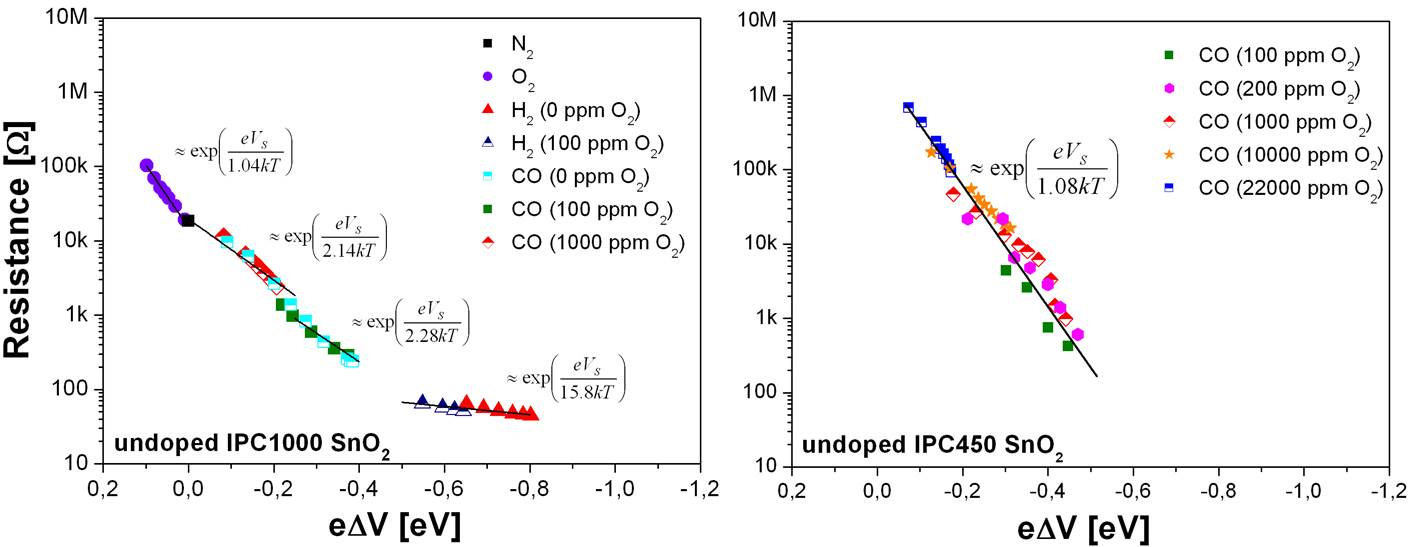
\includegraphics{media/WF450und1000.jpg}
\caption{test}
\end{figure}

    \begin{tcolorbox}[breakable, size=fbox, boxrule=1pt, pad at break*=1mm,colback=cellbackground, colframe=cellborder]
\prompt{In}{incolor}{9}{\boxspacing}
\begin{Verbatim}[commandchars=\\\{\}]

\end{Verbatim}
\end{tcolorbox}


    % Add a bibliography block to the postdoc
    
    
    
\end{document}
